\chapter{参考问题的统一贝叶斯架构及模型选择}
\section{研究背景}
尽管上一章系统分析了多种物理因素对定量脑电中参考效果的影响发现REST和AR相对较好,由于缺乏理论证据二者仍存在较大争议。本章拟提出无穷远参考脑电电位估计的统一贝叶斯线性逆问题架构,认为脑电参考估计可通过最大后验估计求解还可用模型指数评价参考模型的优劣。本章研究的共同统计学架构将为脑电参考问题提供崭新的数理统计学视角。
\begin{figure}[!h]
	\centering
	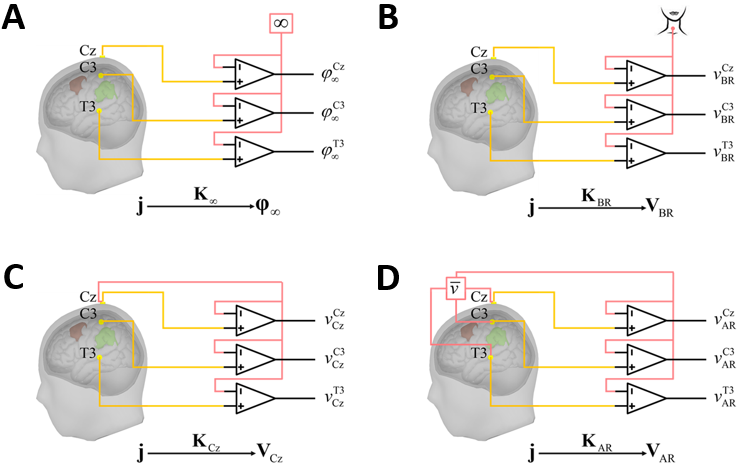
\includegraphics[width=15cm]{pic/Frontier/figure1.png}
	\caption{脑电参考问题图解。脑电记录测量的是活跃电极(黄点)和参考电极(红点)间的电位差。A.无穷远处的参考点;B.身体表面的电极,如脖子;C.头表参考电极Cz;D.所有活跃电极电位的平均值作为平均参考。B-D中的参考用以近似A中的无穷远参考。 不同参考得到不同脑电波形,这就是脑电参考问题。注意神经源活动$\mathbf{j}$相同,不同脑电波形$\mathbf{\phi}_\infty$、$\mathbf{v}_{BR}$、$\mathbf{v}_{Cz}$、$\mathbf{v}_{AR}$可理解为不同参考传递矩阵$\mathbf{K}_\infty$、$\mathbf{K}_{BR}$、$\mathbf{K}_{Cz}$、$\mathbf{K}_{AR}$的结果。}
	\label{3:1}
\end{figure}
脑电的两个主要缺陷,容积传导效应造成的空间混叠和总基于某参考电势测量的固有不确定性\citing{teplan_fundamentals_2002}很大程度上减少了
定量探究脑电活动的能力。脑电记录的固有本质是两个位点的电势差。如图\ref{3:1}所示,人们希望用活跃电极只记录部分脑组织产生的电活动信号,此时相对于具有零活动的中立参考电极。有人认为参考电极应放在无穷远,记录到的电位记为$\mathbf{\phi}_{\infty}$。然而放置参考电极到无穷远好似天线引入大量环境噪声,实际中并不可行。一些研究尝试体表的参考电极以便脑电差分放大器能通过高共模抑制比消除环境噪声。但体表上并无中立的位点,这些提议也失败了。一种物理上中立的参考似乎遥不可及。

非中立参考具有贯穿整个处理步骤直到最终统计结果的影响。既然物理参考不可行,人们希望找到虚拟中立参考$\mathbf{\phi}_{\infty}$的统计学估计量。一种常用的虚拟估计量是图\ref{3:1}D所示的平均参考(AR),它基于:1.内部只有电流源的球面上电势积分为零\citing{goldman_clinical_1950,offner_eeg_1950};2.头表可近似为球面;3.中立参考可通过加权或平均所有电极的活动得到。这
种重参考从所有通道信号减去这种平均信号。然而最近研究\citing{yao_is_2017}发现真实头表面的电位积分不是零,撼动了平均参考的理论基础。
\begin{figure}[!h]
	\centering
	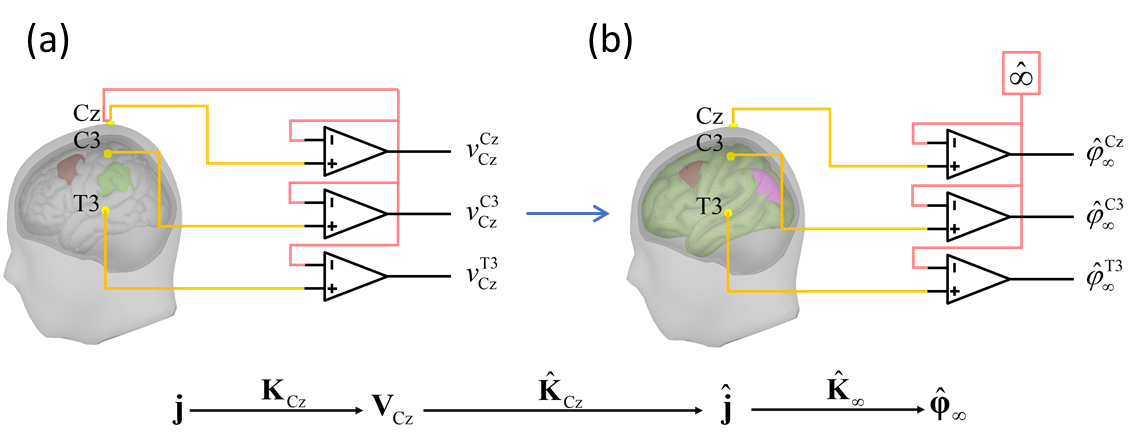
\includegraphics[width=15cm]{pic/Frontier/figure2.png}
	\caption{REST参考变换图解。A.参考到Cz测得的脑电电位$\mathbf{v}_{Cz}$,$\mathbf{j}$和$\mathbf{K}_{Cz}$分别是实际的神经源
	活动和参考到Cz的实际传递矩阵;B.REST先用估计的头模型计算传递矩阵$\hat{\mathbf{K}}_\infty$再转换到$\hat{\mathbf{K}}_{Cz}$, 进而估计等效源$\hat{\mathbf{j}}$, 最后正演等效源活动近似得到无穷远参考下脑电电位$\hat{\mathbf{\phi}}_\infty$。}
	\label{3:2}
\end{figure}
一种更具有生物物理学知识的$\mathbf{\phi}_{\infty}$虚拟估计量可通过图\ref{3:2}所示的零参考REST得到\citing{yao_method_2001}。REST采用头模型和等效源模型估计源活动然后投影源活动到电极上作为对无穷远参考的虚拟估计。REST的早期工作是基于一种简单的球面头模型。脑电功率谱能量地形图\citing{yao_d_comparative_2005}、事件诱发电位成分峰值和潜伏期\citing{li_new_2007}高度依赖参考选择。研究\citing{tian_why_2013}表明听觉视觉刺激诱发电位使用REST的头表统计参数成像比AR更接近LORETA的源定位结果。人们通过仿真得到一些关于REST令人鼓舞的结果。采用球模型仿真,研究\citing{marzetti_l_use_2007,qin_comparative_2010}发现REST比AR得到更好的谱和相干估计。一些仿真和实际数据分析还发现REST采用真实头模型在头表地形图重建\citing{liu_q_estimating_2015}、功能连接\citing{chella_impact_2016}和双谱分析\citing{chella_f_non-linear_2017}上都具有更好效果。

尽管这些结果都支持REST,哪种参考理论更优的问题仍然是激烈争论尚未克服的难题\citing{nunez_rest_2010,kulaichev_optimal_2016}。这是由于仿真研究尽管有用但不足以证明某种参考理论上的绝对优势。除了仿真,找到参考对实际数据最优拟合的证据十分必要。最优模型选择是现代统计学\citing{robert_bayesian_2007}中较多研究的问题,可通过逼近贝叶斯模型证据\citing{konishi_information_2008}的模型选择指数来解决。应用模型选择指数的必要前提是找到脑电参考问题的贝叶斯模型显式表达式。

本章首次将脑电参考问题表示为广义贝叶斯逆问题。这样得到:AR和REST采用相同模型仅区别于无穷远处脑电电位空间协方差的先验,假设电极活动不相关得到AR,如果电极活动是神经源活动经容积导体滤波而相关就得到REST。该理论允许在一致贝叶斯统计架构下比较不同参考估计量。注意REST\citing{yao_method_2001}仅是在理想无噪声情况下推出的。头表电极高度敏感使脑电数据可能具有相当低的信噪比\citing{ferree_scalp_2001,lemm_enhancing_2006,guruvareddy_artifact_2013,bigdely-shamlo_prep_2015},这种无噪声假设并不符合实际。一致的统计学架构允许用正则化技术处理噪声\citing{phillips_empirical_2005,phillips_systematic_2002}。这里发展出REST和AR的正则化版本,分别记为rREST和rAR。AR和REST是rAR和rREST正则化参数分别趋于零时的特例。

为避免按仿真模型求逆的错误\citing{kaipio_statistical_2007},rREST中所用容积传导模型应与正演仿真电位的模型不同。认识REST的容积传导模型匹配问题以避免仿真研究得到负阳性的错误结果。尽管仿真中
REST使用等效源模型,容积传导模型匹配问题仍不可忽略\citing{hu_how_2018}。这里在一致统计架构下进行多种仿真比较AR、REST、rAR、rREST估计$\mathbf{\phi}_\infty$相对误差的性能差异,还在仿真中探究模型准则选择正则化参数的效果。借助古巴人脑计划项目中的89个被试的MRI和脑电数据仿真不同噪声程度的脑电作为基标准,研究表明估计无穷远参考的脑电电位时rREST误差最低,真实容积传导模型改进了REST和rREST的效果。实际应用中被试群体平均的传递矩阵和个体传递矩阵效果接近。基于广义交叉验证的正则化参数选择接近基标准的最佳参数选择。分析89个被试的静息态脑电一致得出rREST具有最优的模型指数。

\section{统一参考估计量}
\subsection{广义脑电参考模型}
脑电总是基于一种时变参考,常被建模为瞬时地从所有电极上减去一个常数。如果测量噪声和大脑信号不同源,可认为有两个不同的参考常数,一个相对于头表脑电信号,另一个相对于电极噪声。在线瞬时记录到脑电信号可表示为:
\begin{equation}\label{eq3.1}
\mathbf{v}=\mathbf{\phi}-\mathbf{1}\times\rho+\mathbf{\epsilon}-\mathbf{1}\times\zeta
\end{equation}
这里$\mathbf{\phi}$是采用中立参考的$N_e$通道干净脑电信号,即上面提到的$\mathbf{\phi}_{\infty}$,其分布是$N(\mathbf{0},\Sigma_{\mathbf{\phi}\mathbf{\phi}})$; $\mathbf{\epsilon}$是电极噪声,其分布为$N(\mathbf{0},\sigma^{2}\mathbf{I}_{N_{e}})$。$\rho$和$\zeta$分别是脑电信号$\mathbf{\phi}$和$\mathbf{\epsilon}$的参考常量。假设$\rho$来自大脑源活动,但$\zeta$可能来自大脑源、非大脑源或二者的混合。由于这些常数不确定,$\mathbf{v}$的参考是未知变量。注意到$\mathbf{\phi}$和$\mathbf{\epsilon}$的其他统计概率分
布也适于该架构。参考过程起到对脑电数据线性变换的作用,相当于对脑电数据矩阵左乘参考变换矩阵。假设参考变换矩阵为$\mathbf{T}=\mathbf{I}_{N_e}-\mathbf{1f}^T$\citing{hu_how_2018},参考变换可写作
\begin{equation*}
\mathbf{v}_{r}=\mathbf{Tv}=\mathbf{T(\phi+\epsilon)}-(\mathbf{I}_{N_e}-\mathbf{1f}^T)\times\mathbf{1}\times(\rho+\zeta)
\end{equation*}
等式$\mathbf{f}^T\mathbf{1}=1$对所有的单极参考均成立,这些单极参考包括如Cz、Fz、Oz的在线记录参考、连接耳参考和平均参考。

因此,广义脑电参考模型为
\begin{equation}\label{eq3.2}
\mathbf{v}_{r}=\mathbf{T\phi+e},\quad\mathbf{e=T\epsilon}
\end{equation}
这里$r$指的是某种参考,$\mathbf{T}$是秩为$N_{e}-1$的矩阵。 因此对$\mathbf{\phi}$的估计转换为欠定的广义线性逆问题。通过最
大后验估计\citing{p_murphy_machine_1991}或最大惩罚似然估计\citing{eggermont_nonparametric_2009}得到目标函数:
\begin{equation}\label{eq3.3}
l=(\mathbf{v}_r-\mathbf{T\phi})^T\Sigma_\mathbf{ee}^+(\mathbf{v}_r-\mathbf{T\phi})+\mathbf{\phi}^T\Sigma_\mathbf{\phi\phi}^+\mathbf{\phi}
\end{equation}
对\eqref{eq3.3}求关于$\mathbf{\phi}$的偏导得
\begin{equation}
\hat{\mathbf{\phi}}=(\mathbf{T}^T\Sigma_\mathbf{ee}^+\mathbf{T}+\Sigma_\mathbf{\phi\phi}^+)^+\mathbf{T}^T\Sigma_\mathbf{ee}^+\mathbf{v}_r
\end{equation}
根据矩阵逆变换引理\citing{hager_updating_1989,tarantola_inverse_2005},$\hat{\mathbf{\phi}}$重新表示为
\begin{equation}\label{eq3.4}
\hat{\mathbf{\phi}}=\Sigma_\mathbf{\phi\phi}\mathbf{T}^T(\mathbf{T}\Sigma_\mathbf{\phi\phi}\mathbf{T}^T+\Sigma_\mathbf{ee})^+\mathbf{v}_r
\end{equation}
此表达式就是重建无穷远参考脑电电位的统一贝叶斯估计量。

为推出\eqref{eq3.4}的显式表达式,假设分布$\Sigma_\mathbf{ee}=\sigma^{2}\mathbf{TT}^T$,$\Sigma_\mathbf{\phi\phi}$服从
如下两种形式。
\subsection{不相关的协方差先验}
\begin{equation}\label{eq3.5}
\Sigma_\mathbf{\phi\phi}=\alpha^{2}\mathbf{I}_{N_e}
\end{equation}
这意味着脑电信号$\mathbf{\phi}$具有所有电极间空间意义上的独立先验,$\alpha^2$是所有电极上脑电信号方差的均值。

将\eqref{eq3.5},$\mathbf{v}_{r}=\mathbf{Tv}$和$\Sigma_\mathbf{ee}=\sigma^{2}\mathbf{TT}^T$代入\eqref{eq3.4}得到
\begin{equation}\label{eq3.6}
\hat{\mathbf{\phi}}=\mathbf{T^{+}Tv}/(1+\sigma^{2}/{\alpha^{2}})
\end{equation}
论文\citing{hu_unified_2018}中附录证明$\mathbf{T^+T}=\mathbf{I}_{N_e}-\mathbf{11}^T/N_e$就是平均参考转换矩阵。定义电极噪声相对头表脑电信号比
例为$nsr_1=\sigma^2/\alpha^2$,同时定义$\mathbf{T}_{ar}=\mathbf{I}_{N_e}-\mathbf{11^T}/{N_e}$,\eqref{eq3.6}可写为
\begin{equation}\label{eq3.7}
\hat{\mathbf{\phi}}=\mathbf{T}_{ar}\mathbf{v}/(1+nsr_1)
\end{equation}
这就是正则化的平均参考(rAR),传统的AR是rAR当$nsr_1=0$时的特例。
\subsection{相关的协方差先验}
\begin{equation}\label{eq3.8}
\Sigma_{\mathbf{\phi\phi}}=\mathbf{K}_{\infty}\Sigma_{\mathbf{jj}}\mathbf{K}_{\infty}^T
\end{equation}
该等式建立了所有电极上脑电电位的相关性,这种相关性是由神经源活动经容积传导效应形成,即假设$\mathbf{\phi}=\mathbf{K}_{\infty}\mathbf{j}$。$\mathbf{K}_\infty$是无穷远参考下的传递矩阵;$\mathbf{j}$是神经源活动的主要电流密度,服从分布$\mathbf{j}\sim{N(\mathbf{0},\beta^2\mathbf{I}_{N_s})}$;$\beta^{2}$是多变量高斯信号$\mathbf{j}$的方差。

定义$\mathbf{K}_r=\mathbf{TK}_{\infty}$并代\eqref{eq3.8}入\eqref{eq3.4}得到
\begin{equation}\label{eq3.9}
\hat{\mathbf{\phi}}=\mathbf{K}_\infty\Sigma_{\mathbf{jj}}\mathbf{K}_r^T(\mathbf{K}_r\Sigma_{\mathbf{jj}}\mathbf{K}_r^T+\Sigma_{\mathbf{ee}})^+v_r
\end{equation}
该表达式就是重建无穷远参考的脑电电位估计量,记为正则化的参考电极标准化技术(rREST)。

可理解该参考变换过程为两个步骤:
\begin{align*}
\qquad\hat{\mathbf{j}}={} &\Sigma_{\mathbf{jj}}\mathbf{K}_{r}^T(\mathbf{K}_{r}\Sigma_{\mathbf{jj}}\mathbf{K}_r^T+\Sigma_{\mathbf{ee}})^+v_r\\
\qquad\hat{\mathbf{\phi}}={} &\mathbf{K}_{\infty}\hat{\mathbf{j}}
\end{align*}
其中步骤一采用传递矩阵$\mathbf{K}_{r}$求解逆问题,该传递矩阵含有和脑电信号$\mathbf{v}_{r}$相同的参考,步骤二正演计算理论的中立
参考脑电电位。步骤一中的$\hat{\mathbf{j}}$是同时求解线性逆问题和参考问题的标准形式。

定义电极噪声对大脑神经源活动信号比例为$nsr_{2}=\sigma^{2}/\beta^{2}$,代$\Sigma_{\mathbf{jj}}=\beta^{2}\mathbf{I}_{N_s}$和$\Sigma_{\mathbf{ee}}=\sigma^{2}\mathbf{TT}^T$到\eqref{eq3.9}得:
\begin{equation}\label{eq3.10}
\hat{\mathbf{\phi}}=\mathbf{K}_{\infty}\mathbf{K}_{r}^{T}(\mathbf{K}_{r}\mathbf{K}_{r}^{T}+nsr_{2}\mathbf{TT^{T}})^{+}\mathbf{v}_{r}
\end{equation}
这就是通过引入等对角线结构$\Sigma_{\mathbf{jj}}$解逆问题来重建无穷远参考脑电电位的解。显然REST\citing{yao_method_2001}$\hat{\mathbf{\phi}}=\mathbf{K}_{\infty}\mathbf{K}_{r}^{+}\mathbf{v}_{r}$是\eqref{eq3.10}中rREST当$nsr_{2}=0$的特例。表\ref{3:bystab}归纳总结出脑电参考估计的统一贝叶斯架构。

\section{参考比较}
如表\ref{3:bystab}所示,如果电极噪声为零或不采用正则化技术,AR和REST分别是rAR和rREST的特例。本节转换广义参考模型到标准脊回归形式采用统计模型准则比较参考估计量。

\bigskip
\bigskip
\bigskip
\begin{table}[!h]
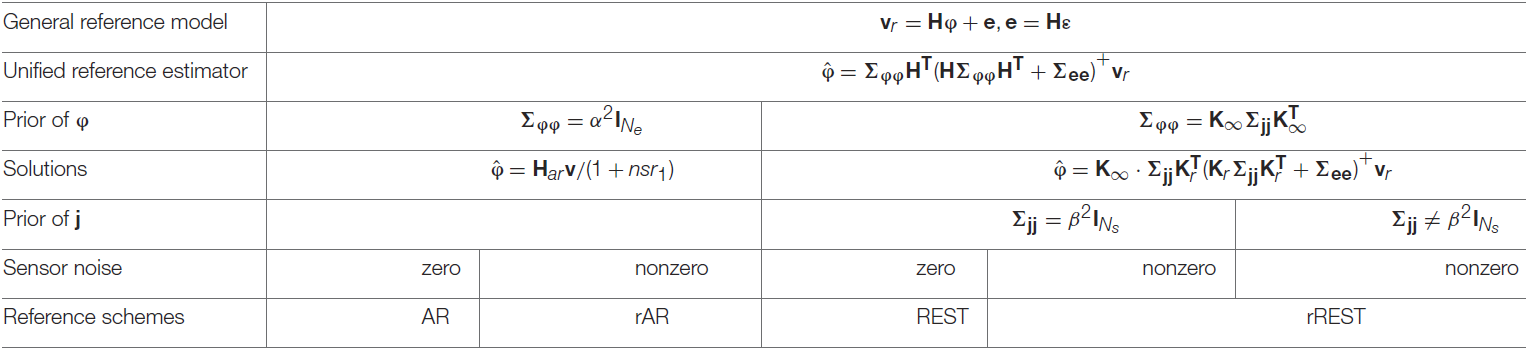
\includegraphics[width=\linewidth]{pic/Frontier/bayesiantab.png}
\caption{脑电参考估计的统一贝叶斯架构。}
\label{3:bystab}
\end{table}
\bigskip

\subsection{标准回归形式}
参考估计的目标函数\eqref{eq3.3}等价于广义脊回归形式\citing{chung_optimal_2014}:
\begin{equation}\label{eq3.11}
\hat{\mathbf{\phi}}(\lambda)=arg\min_{\mathbf{\phi}}{\lVert\mathbf{v}_{r}-\mathbf{T\phi}\rVert_{M}^{2}+\lambda\lVert\mathbf{L\phi}\rVert_2^2}
\end{equation}
这里$\lambda\geq{0}$是正则化参数,$\mathbf{L}$是正则化矩阵。这里称$\lambda$和$\mathbf{L}$的作用分别为参数正则化和结构正则化。脊回归是Tikhonov正则化的统计学名字\citing{hoerl_ridge_1970}。脊回归的广义与标准形式区别在正则化矩阵$\mathbf{L}$是否为单位阵、失匹配项是否为欧式模\citing{chung_optimal_2014}。重定义$\mathbf{\phi^\prime=L\phi}$转换正则化矩阵为单位阵同时$\mathbf{e^\prime=D^{T}U^{T}e}$(分解$\mathbf{TT^{T}=USU^{T}}$和$\mathbf{S}^+=\mathbf{DD}^T$)以转换失匹配项从Mahalanobis模为欧式模。最终标准脊回归形
式为
\begin{equation}\label{eq3.12}
\hat{\mathbf{\phi}}^\prime(\lambda)=arg\min_{\mathbf{\phi}^\prime}{\lVert{\mathbf{v}_r^\prime-\mathbf{T^\prime\phi^\prime}}\rVert_2^2+\lambda\lVert{\mathbf{\phi}^\prime}\rVert_2^2}
\end{equation}
这里$\mathbf{v}^\prime_r=\mathbf{D^TU^Tv}_r$,$\mathbf{T}^\prime=\mathbf{D^TU^TTL}^+$。然后,$\mathbf{\phi}^\prime$关于$\mathbf{v}^\prime_r$的后验均值是
\begin{equation}\label{eq3.13}
\hat{\mathbf{\phi}}^\prime=(\mathbf{T^{\prime^T}}\mathbf{T}^\prime+\lambda\mathbf{I}_{N_e})^+\mathbf{T^{\prime^T}}\mathbf{v}^\prime_r
\end{equation}
那么关于$\mathbf{\phi}$的估计就是$
\hat{\mathbf{\phi}}=\mathbf{L}^+(\mathbf{T}^{\prime^T}\mathbf{T}^\prime+\lambda\mathbf{I}_{N_e})^+\mathbf{T}^{\prime^T}\mathbf{v}^\prime_r$,该等式等价于\eqref{eq3.10}。
\subsection{模型选择准则}
因为脊回归是一种线性估计量($\hat{\mathbf{v}}^\prime_r={\mathbf{Pv}^\prime_r}$),$\mathbf{P}=\mathbf{T}^\prime(\mathbf{T^{\prime^T}}\mathbf{T}^\prime+\lambda\mathbf{I}_{N_{e}})^{+}\mathbf{T^{\prime^T}}$作为投影(hat)矩阵。残差平方和(residual sum square error,RSS)定义为
\begin{equation}
RSS=\sum_{t=1}^{N_{t}}\lVert\mathbf{v}^\prime_{rt}-\mathbf{T}^\prime\hat{\mathbf{\phi}}^\prime_t\rVert_2^2
\end{equation}
这里$\mathbf{v}^\prime_{rt}$和$\hat{\mathbf{\phi}}^\prime_t$是$t^{th}(t=1,...,N_t)$时间点的$\mathbf{v}^\prime_r$和$\hat{\mathbf{\phi}}^\prime$,$N_t$是整个脑电记录的时间点数。

基于\eqref{eq3.12}标准脊回归形式,用模型选择指数广义交叉验证(GCV)\citing{chung_optimal_2014}、Akaike信息准则(AIC)和Bayesian信息准则(BIC)\citing{konishi_information_2008}比较表\ref{3:bystab}中的参考估计量。定义自由度
\begin{equation}
DF=\Tr(\mathbf{P})=\sum_{i=1}^{N_{e}}\dfrac{s_i}{s_i+\lambda}
\end{equation}
这里$s_i$是$\mathbf{T}^{\prime^T}\mathbf{T}^\prime$的特征值。因为脑电参考相当于单个时刻点所有电极上加减一个时变常数,这种瞬时效应造成时域动力学失真。为探究参考差异将模型选择指数
从单时刻点近似推广到全局记录。预定义$N_{et}=N_eN_t$,GCV、AIC和BIC可表示为
\begin{align}
GCV(\lambda)={} &RSS/(N_{et}-DF)^2\label{eq3.14}\\
AIC(\lambda)={} &N_{et}\log(RSS/{N_{et}})+N_t\cdot{2}\cdot{DF}\label{eq3.15}\\
BIC(\lambda)={} &N_{et}\log(RSS/{N_{et}})+N_t\cdot{DF}\cdot{\log(N_{et})}\label{eq3.16}
\end{align}
注意到单个时刻点下GCV、AIC和BIC分别是\eqref{eq3.14}、\eqref{eq3.15}和\eqref{eq3.16}在$N_t=1$时的特例。
\subsection{正则化参数}
正则化参数$\lambda$平衡了数据模型拟合效果与无穷远参考下脑电信号的先验约束。人们可能尝试迭代交互估计层级贝叶斯超参数\citing{mackay_bayesian_1992,trujillo-barreto_bayesian_2004}。但这可能对rREST有效对rAR却不奏效,因为rAR中的噪声项会因独立相同协方差先验被同化为\eqref{eq3.6}中的干净脑电信号。AR的非凸目标函数无法收敛到全局或局部最优点。这里采用搜索策略探究DF、GCV、AIC和BIC如何随$\lambda$变化\citing{phillips_empirical_2005}。方法是画出DF随$\lambda$以及GCV、AIC和BIC随DF的变化曲线。\eqref{eq3.7}和\eqref{eq3.10}的理论结果表明rAR的最优$\lambda$接近$nsr_1$,rREST的接近$nsr_2$。容积传导效应相当于低通时空滤波,会导致$nsr_2\ll{nsr_1}$\citing{srinivasan_r_spatial_1998,stinstra_volume_1998,srinivasan_methods_1999,nunez_electric_2006}。假设rREST信噪比区间
是[35, 10]dB,rAR的信噪比区间是[30, −10]dB,用采样算法随机生成1000个$\lambda$,对于rREST和rAR分别从$10^{-3.5}$到0.1和从$10^{-3}$到10。

为比较参考估计量,在仿真中设最优正则化参数,该参数下得到相对于基准电位的最小误差。还能比较模型选择准则GCV、AIC和BIC选择正则化参数的效果。因为基准脑电数据在实际脑电数据分析中未知,找到合适$\lambda$更困难,当模型选择准则达到全局最优时的参数$\lambda$视为真实脑电数据中该模型选择准则的最优$\lambda$值。

研究\citing{yao_method_2001}建议使用REST时避免采用正则化参数以免丢失高频信息。论文\citing{zhai_y_and_yao_d_study_2004}中提出使用REST时可采用截断奇异值的方法抑制电极噪声。因此本章先验地
选择REST中推荐的截断参数0.05,但在rREST中仍采用模型选择准则。
\subsection{正则化矩阵}
正则化矩阵$\mathbf{L}$的选择依赖于无穷远电位的先验协方差结构。如表\ref{3:bystab}所示AR和rAR的先验协方差是$\Sigma_{\mathbf{\phi\phi}}=\alpha^{2}\mathbf{I}_{N_e}$,REST和rREST的先验协方差是$\Sigma_{\mathbf{\phi\phi}}=\mathbf{K}_{\infty}\Sigma_{\mathbf{jj}}\mathbf{K}_{\infty}^T$。 因此$\mathbf{L}$的选择是:

对于AR和rAR,$\mathbf{L}_{ar}=\mathbf{I}_{N_e}$;

对于REST和rREST,
\begin{equation}\label{eq3.17}
\mathbf{L}_{rt}=[(\mathbf{K}_\infty\mathbf{K}_\infty^T)^+]^{1/2}
\end{equation}

$\mathbf{K}_\infty$的详细讨论见下一节。$\mathbf{L}_{rt}$中生物物理信息的正则化程度与传递矩阵对容积传导模型的近似程度正相关。
\subsection{容积传导模型}
无论仿真脑电还是真实脑电都可理解为从传递矩阵得到,本节研究rREST可能涉及到的容积传导模型匹配问题,rREST的传递矩阵多大程度上可能偏离实际真实传递矩阵。几种传递矩阵是频繁采用的标准球形传递矩阵(SLF)、最精确的基于个体被试MRI结构数据的个体传递矩阵(ILF)和被试群体平均的传递矩阵(ALF)。因仿真中可知源是否激活,这里还研究个体被试稀疏源的传递矩阵(sILF)。
\subsubsection{球形传递矩阵 (SLF)}
$\mathbf{K}_{\infty}^{s}$基于三层同心球面模型生成,三层分别是大脑皮层、颅骨、头表,相对传导率分别为1、0.0125和1,头皮和颅骨内外表面相对半径分别是1.0、0.87和0.92。源空间由2600个均匀垂直于皮层表面半径为0.86的离散偶极子和400个均匀垂直于$z=-0.076$的水平断面偶极子组成。这里传导率、半径和坐标值都不是实际测量值而是层层间传导率、半径的相对比例,以及单位球面空间中的坐标值\citing{yao_method_2001,hu_how_2018}。
\subsubsection{个体传递矩阵(ILF)}
$\mathbf{K}_{\infty}^i$通过归一化定义为
\begin{equation*}
\mathbf{K}_\infty^i=\mathbf{K}_\infty^{iraw}/{[\Tr(\mathbf{K}_\infty^{iraw}\mathbf{K}_\infty^{{iraw}^T})]^{1/2}}
\end{equation*}
这里$\mathbf{K}_{\infty}^{iraw}$是与古巴人类脑影像计划\citing{uludag_latin_2009,valdes-hernandez_white_2010,hernandez-gonzalez_multimodal_2011,bosch-bayard_3d_2012}中接受脑电采集的第$i^{th}=1,...,N_b$被试相匹配的原始个体传递矩阵。原始的个体传递矩阵通过基于分割结构MRI数据为大脑皮层的CIVET流程\citing{ad-dabbagh_civet_2006}和有限元方法估计得到。大脑皮层表面由6003个顶点和11998个面组成。总共6003个偶极子源分布在各个顶点并垂直于皮层表面。对不同被试个体的传递矩阵归一化便于进行被试间组分析。

\subsubsection{平均传递矩阵(ALF)}
$\mathbf{K}_{\infty}^a$是$N_b$个被试的所有归一化个体传递矩阵的平均,表示为:
\begin{equation*}
\mathbf{K}_{\infty}^a=\frac{1}{N_b}\sum_{i=1}^{N_b}\mathbf{K}_{\infty}^i
\end{equation*}

\subsubsection{稀疏化个体传递矩阵(sILF)}
只有仿真可知源的稀疏度所以只在仿真中使用,先转换为个体传递矩阵(ILF)再通过如下计算获得
\begin{equation*}
\mathbf{K}_{\infty}^{si}=[\mathbf{K}_{\infty}^{iraw}\circ\mathbf{W}_i]/{[\Tr(\mathbf{K}_{\infty}^{iraw}\circ\mathbf{W}_i\mathbf{W}_i^T\circ{\mathbf{K}_{\infty}^{iraw}}^T)]^{1/2}}
\end{equation*}
这里$\circ$是矩阵的Hadamard积;$\mathbf{W}_i$是和$\mathbf{K}_{\infty}^{iraw}$有相同大小的二值权重矩阵;在未激活的神经源对应列的元素权重为零,其它列为1。 仿真中两个小块的位置信息被引入到rREST对待估计无穷远参考下脑电电位的空间协方差中,而非采用$\ell_0$或$\ell_1$来稀疏大脑神经源信号$\mathbf{j}$,设个体传递矩阵中对应非激活源的元素为零以间接约束大脑神经源信号。

\section{结果}
\subsection{仿真比较与模型选择}
\subsubsection{脑电生成}
仿真思路是按如下正演计算公式:
\begin{equation}\label{eq3.18}
\begin{aligned}
\mathbf{v}_r& =\mathbf{T\phi}+\mathbf{T\epsilon},\mathbf{\phi}=\mathbf{K}_{\infty}^{iraw}\mathbf{j}\\
SNR& =10\log_{10}(\alpha^2/\sigma^2)
\end{aligned}
\end{equation}
这里$\mathbf{v}_r$是基于单极参考仿真出的脑电电位;不失一般性,线性结合向量$\mathbf{f}=[0,...,0,1]^T$除最后一个元素为1其他均为零
;如图\ref{3:3}所示神经源$\mathbf{j}$中两个源块包含150个激活偶极子,满足四阶双变量自回归模型;信噪比SNR是头表脑电信号与传感器电
极噪声方差之比,以分贝dB为单位。
\begin{figure}[!h]
	\centering
	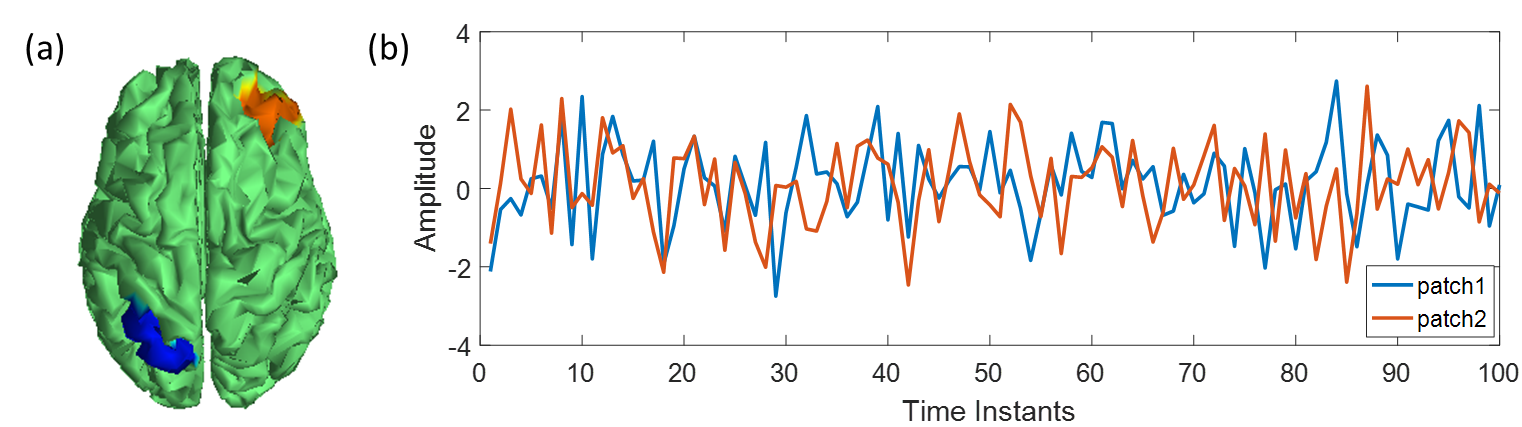
\includegraphics[width=15cm]{pic/Frontier/figure3.png}
	\caption{仿真脑电所用的神经源活动示意。A.两个神经源块的位置;B.两个神经源块的神经活动。}
	\label{3:3}
\end{figure}
用古巴人脑计划数据库中的89个被试的个体传递矩阵$\mathbf{K}_{\infty}^{iraw}$,仿真每组脑电数据是89被试$\times$58通道$\times$5120时刻点。共仿真得到数据集A:4组数据,信噪比SNR组内相同组间不同,数据集B:1组数据,SNR对所有被试都不同。仿真给出基于中立
无穷远参考的脑电电位基标准,这样能用脑电电位误差直观比较参考效果。每个被试脑电数据的相对误差定义为
\begin{equation}\label{eq3.19}
RE=\lVert\hat{\mathbf{\phi}}-\mathbf{\phi}\rVert^2_F/{\lVert\mathbf{\phi}\rVert^2_F}
\end{equation}
这里$\mathbf{\phi}$是仿真脑电电位基标准,$\hat{\mathbf{\phi}}$是参考估计出的脑电电位。

\subsubsection{参考估计量的相对误差}
\begin{figure}[!h]
	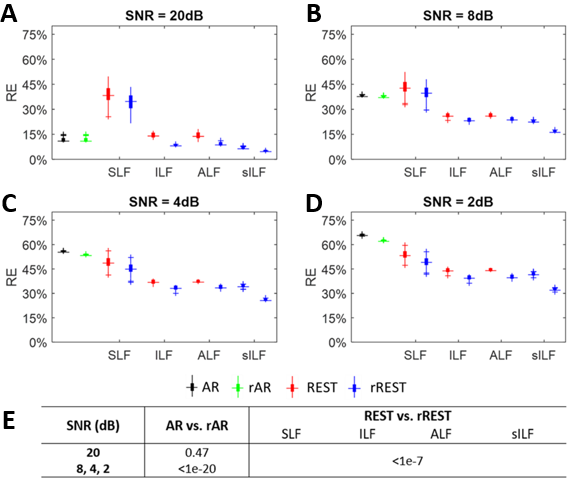
\includegraphics[width=15cm]{pic/Frontier/figure4.png}
	\caption{参考估计量的相对误差。A-D.用柱状图表示信噪比为20、8、4和2dB时电位相对误差;REST和rREST中测试的容积传导模型包含球面
	传递矩阵(SLF)、个体传递矩阵(ILF)、被试群体平均传递矩阵(ALF)和稀疏化个体传递矩阵 (sILF);E.不同信噪比和传递矩阵情况下传统参考
	(AR, REST)和正则化参考(rAR, rREST)间的统计p值。}
	\label{3:4}
\end{figure}
仿真数据集A中具有4组数据,SNR分别为20、8、4、2dB。图\ref{3:4}中A–D表示REST和rREST的相对误差,分别对应四种传递矩阵的情况 (SLF、ILF、ALF和sILF) 。 黑绿红蓝柱状图分别表示AR、rAR、REST和rREST的相对误差。从图\ref{3:4}A–D的柱状图可看出正则化参考rAR、rREST的相对误差总小于传统参考AR、REST的相对误差。用非配对型t检验检查非正则化参考AR、REST与正则化参考rAR、rREST间的差异。图\ref{3:4}E列出AR与rAR间的统计显著性p值及使用各种传递矩阵时REST与rREST间的显著性水平。除AR与rAR在SNR=20dB时,p值都非常小(<1e-7)。采用正则化,从REST到rREST的相对误差下降比AR到rAR的下降更明显。尤其是使用稀疏化个体传递矩阵正则化比球面传递矩阵、个体传递矩阵、被试平均的传递矩阵更有效。 这是因为引入神经源活动的稀疏先验信息到协方差结构中。相比,使用最简单的球面传递矩阵,当SNR=20或8dB时rREST的相对误差似乎比AR大,在所有参考中REST最差。把稀疏化个体传递矩阵的相对误差和球面传递矩阵时rREST的相对误差与球面传递矩阵REST的相对误差比较,且所有测试$\lambda$中得到最小相对误差那个为最优$\lambda$,发现使用恰当协方差进行结构正则化比选择最优$\lambda$进行参数正则化更有效。稀疏化个体传递矩阵rREST的相对误差比其他所有参考相对误差都小,意味着结构正则化结合参数正则化会达到最优效果。另外引入更大传感器电极噪声使SNR从20dB降低到2dB,rAR的相对误差从少于15\%增加到高于60\%,相比除去球面传递矩阵的情况,rREST的相对误差从4.1\%增加到40\%。
这些结果表明:1.除了AR和rAR在SNR=20dB时,AR、rAR和用球面传递矩阵的REST和rREST无法重建无穷远参考下的脑电信号,此时相对误差很大;2.REST和rREST依赖容积传导模型;3.更严格的正则化rREST取得更好效果;4.被试群体平均传递矩阵REST和rREST的相对误差达到和被试个体传递矩阵几乎一致的效果;5.rAR可能没有去噪效果。 总之,当SNR非常高$\geq$20dB时AR和rAR可作为rREST的替代选择,但有接近准确容积传导模型时rREST应作为估计无穷远参考脑电电位的首选。
\begin{figure}[!h]
	\centering
	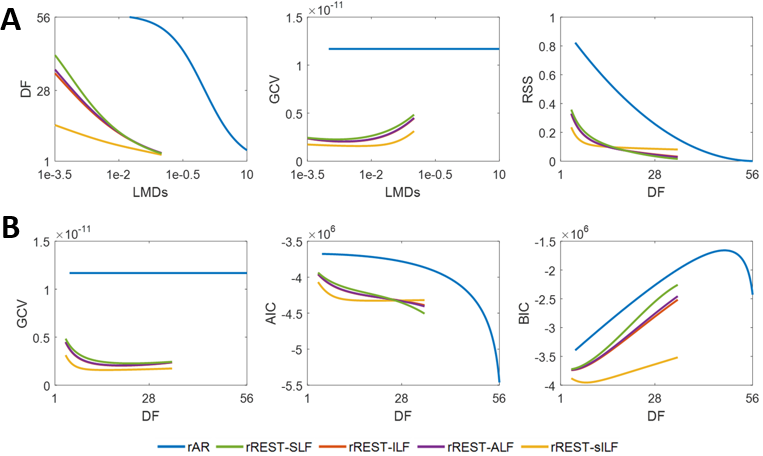
\includegraphics[width=15cm]{pic/Frontier/figure5.png}
	\caption{用仿真数据进行模型选择。DF、RSS、GCV、AIC和BIC是利用不同头模型仿真出89例脑电数据上的平均结果,每一例脑电数据的信噪比不同,信噪比范围[5, 20]dB。A.DF和GCV随LMD的变化曲线,RSS随DF的变化曲线;B.随DF变化的模型准则曲线(GCV、AIC和BIC)。 DF:自由度,RSS:残差平方和,GCV:广义交叉验证,AIC:Akaike信息准则,BIC:Bayesian信息准则,SLF:球形传递矩阵,ILF:个体实际传递矩阵,ALF:个体实际传递矩阵的平均,sILF:稀疏化个体传递矩阵。}
	\label{3:5}
\end{figure}

\subsubsection{用仿真数据进行模型选择}
这里仿真数据集B进行模型选择,数据集B中89个样本被设置均匀分布在[5, 20]dB的SNR值以模拟实际脑电记录中被试间的不同噪声程度。图\ref{3:5}中结果允许通过模型准则选择最优参考。自由度DF、残差平方和RSS
以及模型选择准则(GCV、AIC、BIC)是89个数据样本逐一关于所有检测正则化参数$\lambda$的平均。图\ref{3:5}A中曲线表示DF和GCV如何随$\lambda$变化以及RSS如何随DF变化。容易看出rREST的DF总比rAR的DF小。这意味着rREST比rAR采用更简单模型重建无穷远参考下的脑电信号但采用更切合实际的先验信息进行正则化。rREST比rAR低的RSS表明rREST重建的脑电信号相对于rAR重建的脑电信号更接近于仿真基标准。图\ref{3:5}B的曲线表示模型选择准则(GCV、AIC、BIC)随着DF变化。显然rREST的模型选择准则总比rAR小。普遍更低的模型选择准则值给出rREST比rAR更优的证据。
\begin{figure}[!h]
	\centering
	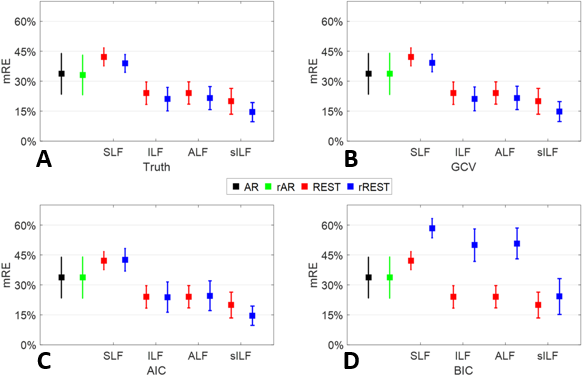
\includegraphics[width=15cm]{pic/Frontier/figure6.png}
	\caption{正则化参数选择。每个方形和误差条(error bar)是用不同信噪比和头模型仿真的89例脑电数据上误差和标准偏差在89例被试间的平
	均。A.用最小相对误差选出的最优$\lambda$值作为基准的结果,B–D.分别用最小GCV、AIC和BIC值选出$\lambda$值的结果。}
	\label{3:6}
\end{figure}

\subsubsection{正则化参数}
选择最优正则化参数$\lambda$对rREST至关重要。图\ref{3:6}表示模型选择准则GCV、AIC和BIC选出的$\lambda$和基标准正则化参数的接近程度,基标准正则化参数由基于仿真数据集B参考前后相对误差最小的准则
选出。被试个体上通过基标准和模型选择准则识别出最优$\lambda$。图\ref{3:6}B–D中平均相对误差(mRE)和标准偏差和图\ref{3:6}A相比发现GCV得到与基标准几乎一致的结果,说明GCV是正则化参数选择的最优准则
。AIC不如GCV,因为除稀疏化个体传递矩阵rREST、正则化参考(rAR, rREST)具有和普通参考(AR, REST)相同或更大的平均相对误差和标准偏差;BIC最不适于选择正则化参数,因为所有的正则化参考得到比传统参考(AR、REST)更大的平均相对误差和标准偏差。

\subsection{用真实数据进行模型选择}
这里用古巴人脑计划数据库中89个被试的脑电数据比较参考估计量。脑电记录实验经过相关伦理道德委员会的批准,被试都签有知情同意书。脑电采集使用10-10电极放置系统58通道,采样率200Hz,每个被试在交替睁闭眼的静息状态下记录2.5到5分钟。图\ref{3:7}是真实脑电数据示例。为在所有被试上比较参考效果,脑电数据进行归一化:$\mathbf{v}_r=\mathbf{v}_r^{raw}/\lVert\mathbf{v}_r^{raw}\rVert_F$。对每个被试数据分别用被试个体传递矩阵、稀疏化个体传递矩阵、平均传递矩阵和球面传递矩阵进行REST变换,并计算GCV、AIC和BIC模型选择准则。模型选择准则又在89个被试间进行平均。 
\begin{figure}[!h]
	\centering
	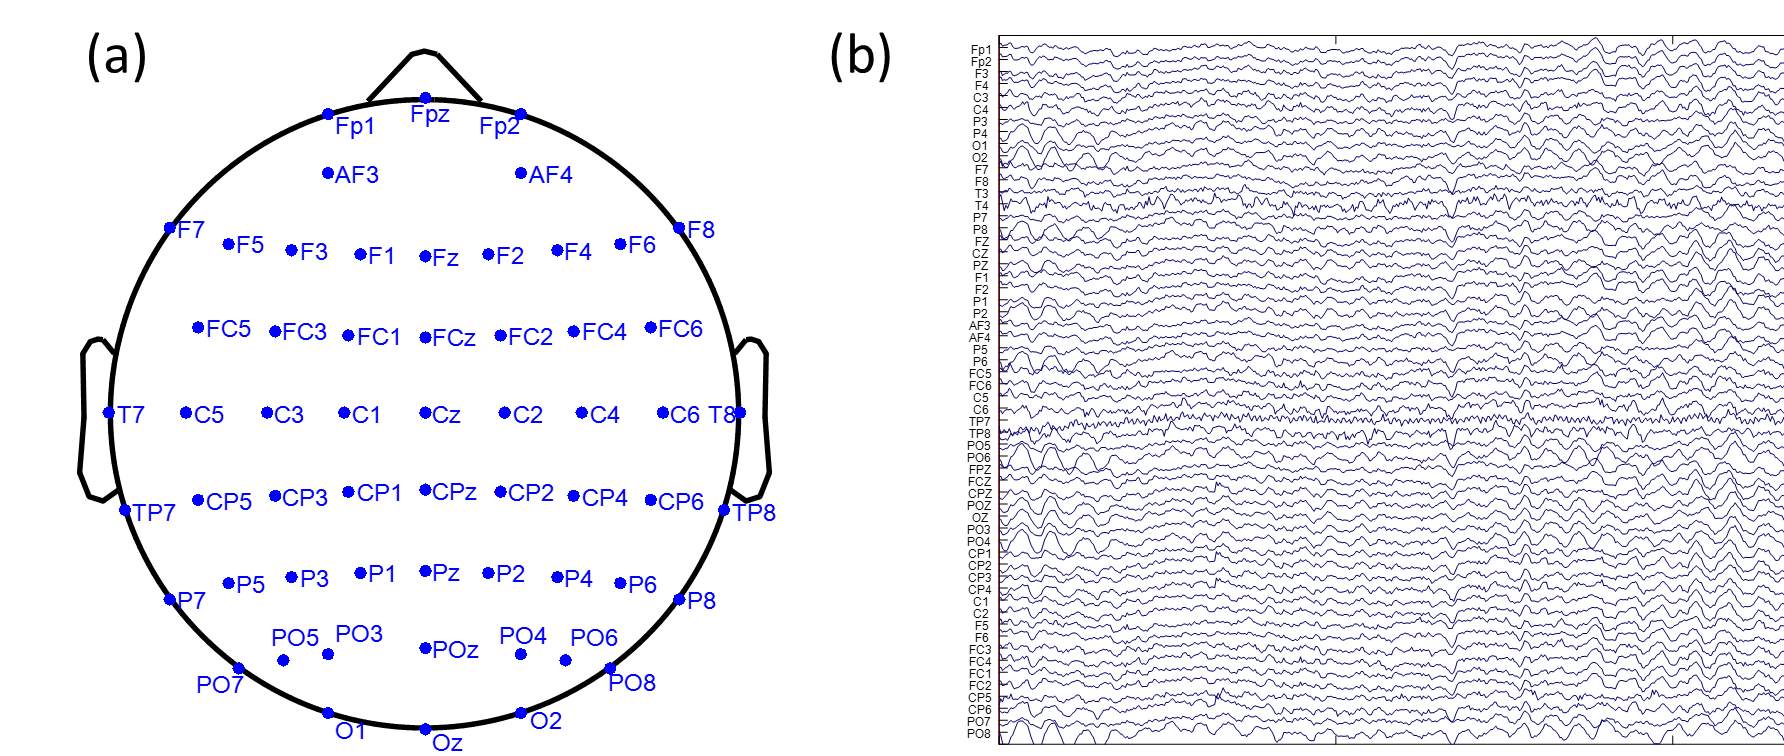
\includegraphics[width=15cm]{pic/Frontier/figure7.png}
	\caption{真实脑电数据示例。A.电极分布图;B.一段真实脑电数据示例。}
	\label{3:7}
\end{figure}

为验证rREST比rAR更优,在89个被试的实际脑电数据中采用与仿真中参考比较相似的分析步骤。图\ref{3:8}中表示DF和GCV随正则化参数$\lambda$变化以及RSS和模型选择准则(GCV、AIC和BIC)随DF变化曲线。
图中画出的DF、RSS和模型选择准则是89个被试逐一分析后被试间平均的结果。因为参考转换矩阵$\mathbf{T}$和正则化参数$\lambda$的区间和仿真中一致,图\ref{3:8}A中DF随$\lambda$的变化曲线和图\ref{3:5}A中完全一致。图\ref{3:8}B中更低的RSS和模型选择准则曲线说明真实数据分析验证了仿真结果:1.rREST重建的脑电信号比rAR重建的信号RSS更低;2.除DF≈28时rREST和rAR有几乎一样的BIC,
rREST比rAR都有更小的GCV、AIC和BIC。因图\ref{3:6}中GCV是仿真中选择正则化参数$\lambda$的最优准则,建议当实际数据基标准未知时尝试采用GCV选择$\lambda$值。图\ref{3:8}A中的中间曲线是GCV随$\lambda$值变化。对于rREST,GCV在$\lambda=10^{-2}$或DF=10附近达到全局最小。因此可推断在实验数据组分析中可能通过最小GCV找到最优正则化参数,这为应用rREST时选择最优$\lambda$提供了先验。图\ref{3:6}说明对每个被试的脑电都用GCV选择正则化参数是没问题的,但rAR的GCV曲线好像是常数直线,这是因为rAR是非凸解就很难找到恰当$\lambda$。这些结果表明真实脑电数据分析验证了rREST比rAR更优,可在GCV
曲线全局最小值处选出rREST的最优正则化参数。
\begin{figure}[!h]
	\centering
	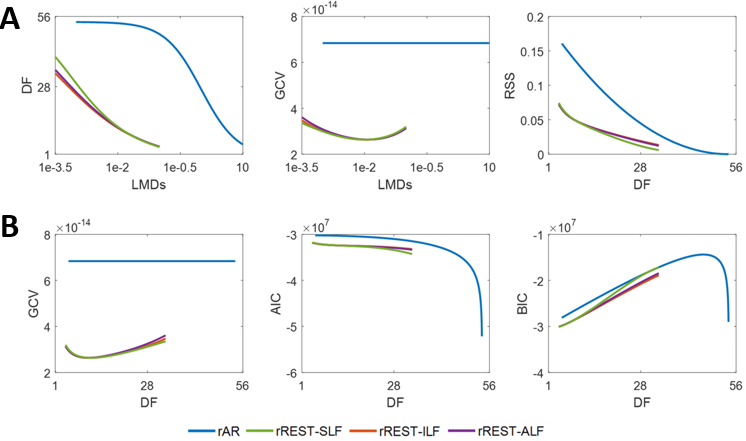
\includegraphics[width=15cm]{pic/Frontier/figure8.png}
	\caption{用真实脑电进行模型选择。 DF、RSS、GCV、AIC和BIC是89例真实脑电数据上的平均。A.DF和GCV随LMD变化曲线,RSS随DF变化曲线; B.模型选择准则GCV、AIC和BIC随DF变化曲线。DF:自由度,RSS:残差平方和,GCV:广义交叉验证,AIC:Akaike信息准则,BIC:Bayesian信息准则,SLF:球形传递矩阵,ILF:个体被试实际的传递矩阵,ALF:被试群体实际传递矩阵的平均。}
	\label{3:8}
\end{figure}

\section{讨论}
REST的理论基础尚未从数理统计角度被研究过。早于REST,平均参考就被微状态分析\citing{khanna_microstates_2015}普遍采用,也作为逆问题中参考选择的终解\citing{rd_pascual-marqui_review_1999,pascual-marqui_standardized_2002,pascual-marqui_discrete_2007,pascual-marqui_assessing_2011}。当前AR和REST依然存在较大争论,其理论差异尚不明确\citing{nunez_rest_2010}。尽管关于二者有许多对比研究,但这些均没有提供明确的理论证据以支持其一\citing{qin_comparative_2010,
chella_impact_2016,chella_f_non-linear_2017,lei_x_and_liao_k_understanding_2017}。最近D. Yao的理论结果证明AR的物理学假设,头皮上脑电信号的平均作为对大脑参考信号的消除一般是错的\citing{yao_is_2017}。但仅从生物物理学角度解决参考问题可能比较困难,采用数理统计学模型进行参考选择也十分必要。

本章把无穷远参考下电位估计和参考选择看作线性逆问题,用贝叶斯技术求解。AR和REST是具有不同脑电电位空间协方差先验分布的特例。引入电极噪声到参考模型把无穷远参考下电位估计和去噪结合起来,基于最大后验估计衍生出正则化rAR和rREST。最后将参考估计转换为标准脊回归形式进行参考模型选择。仿真和实际脑电数据分析都说明:1.正则化对同时解决参考问题和去噪很重要;2.正则化rAR、rREST比非正则化参考AR、REST更优;3.rREST优于rAR;4.应用rREST到真实脑电数据,广义交叉验证是选择正则化参数的有效指标。支持rREST的根本证据是89例真实脑电数据中rREST具有更小的广义交叉验证值。这是首次利用先验和类似贝叶斯模型
证据的信息准则比较参考。

证明AR并非参考问题的终解\citing{pascual-marqui_assessing_2011},只是统一参考估计量中不相关先验和无噪声情况的特例。Pascual等\citing{pascual-marqui_assessing_2011}利用完全无噪声或测量噪声协方差矩阵是单位阵的假设推出AR。参考问题被AR解决,AR被以为是参考过程的最佳拟合。如果参考过程不仅存在脑电信号也存在测量噪声中,AR就无法推出。因为逆问题不取决于参考电极变换,AR和单极参考可用来转换传递矩阵,式\eqref{eq3.9}中rREST的步骤一表示解逆问题前需要转换传递矩阵和脑电记录具有相同的参考。

REST因其合乎逻辑的理论基础引人注意\citing{yao_method_2001,kayser_j_and_tenke_c_e_search_2010,nunez_rest_2010}。然而普通REST的一些结果并非都比AR好\citing{yao_method_2001,hu_how_2018}。垂直于大脑皮层或者浅表层偶极子源活动时普通REST比AR更有效,但水平断面或深层偶极子活动时并非如此。这些发现是由于普通REST的协方差结构来自球形容积传导体和等效分布偶极子层\citing{yao_equivalent_2003},即径向分布于皮层薄片栅格上的源\citing{yao_method_2001}。本章检测了更多类型的真实容积传导模型,且仿真研究是基于多个皮层上的小块源。结果表明切合实际的容积传导模型和源空间下参考估计量并非好很多,实际中REST在多数情况比AR更优。

这里强调多种源模型可能性和广义逆问题概念。因为REST属于广义逆问题,多种源\citing{daunizeau_bayesian_2006}和分布在大脑容积体素的每个栅格点上的三维分布源\citing{michel_eeg_2004}均适合REST\citing{yao_d_high-resolution_2000}。但广义逆不尽相同,将来可能探究如何应用不同源模型到REST中。

测试发现REST和rREST都依赖容积传导模型以及足够逼真容积传导模型的重要性。这与论文\citing{hu_how_2018,liu_q_estimating_2015}的结果一致。论文\citing{liu_q_estimating_2015}表明实际容积传导模型对传统REST较重要。研究\citing{hu_how_2018}发现传统REST依赖容积传导模型但不精确或轻微扰动的传递矩阵不会影响REST效果太多。仿真发现更优容积传导模型和源会带给参考估计量更好的效果。sILF在rREST的容积传导模型测试中得到最小的相对误差是因为先验的sILF匹配正演计算。仿真研究唤起对rREST先验准确性的认识,越切合实际越好。毋庸置疑只能尽可能逼近实际,将来可能通过贝叶斯模型平均\citing{trujillo-barreto_bayesian_2004}考虑先验不确定性。估计个体被试传递矩阵需要的被试结构MRI数据一般不易得到且计算耗时。被试群体平均的传递矩阵实现了和个体被试传递矩阵几乎相同的效果,验证
了没有个体磁共振数据时用近似头模型\citing{valdes-hernandez_approximate_2009}代替的想法。rREST的关键之一是正则化参数选择,这也是统计学习研究的热点之一\citing{konishi_information_2008}。仿真和真实脑电数据结果都表明广义交叉验证是简单有效的指标。实际中应采用广义交叉验证准则选择单个被试脑电记录的正则化参数。

本章主要贡献是提出参考估计的统一贝叶斯线性逆问题架构,把电极噪声模拟为脑电生成模型的一部分。AR和REST是线性逆问题的特例,前者采用空间独立先验后者采用容积传导形成的空间相关先验。正则化的参考估计量rAR和rREST可同时进行参考估计和去噪。采用模型选择准则不仅可用于选择超参数还可用于比较参考模型。被试群体的平均传递矩阵可在实际中替代个体传递矩阵构造近似最优的参考估计量。

对存在的不足可能将抑制噪声与参考估计相结合,通过鲁棒统计学似然函数消除离群值\citing{huber_robust_1981}。考虑更多生物物理先验更有效地分离脑电信号和噪声,也可以对比不同稀疏度源模型的协方差结构\citing{paz-linares_spatio_2017}。模拟时域的自相关为状态空间模型并通过卡尔曼滤波器\citing{galka_solution_2004}估计出动力学后验信息。该统计学架构还可扩展到事件诱发电位的信号处理中\citing{carbonell_random_2004}。

\section{本章小结}
本章统一脑电参考问题为逆问题并通过贝叶斯求解,是脑电参考问题的创新方案,允许用正则化方法估计无穷远参考下的电势。证明REST和AR是统一贝叶斯估计量的特例,二者区别于脑电电势的空间协方差先验。引入去噪到参考估计中并采用模型指数选择最优参考估计量。rREST和rAR分别优于传统REST和AR,rREST无论在仿真还是真实数据上都最优。推荐选择被试个体或群体平均的传递矩阵作为容积传导模型。rREST是REST改进的估计量,有望在临床实践中得以使用。